\chapter{Exercise Recommendation System Based on Knowledge State}

% **************************** Define Graphics Path **************************
\ifpdf
  \graphicspath{{Chapter4/Figs/Raster/}{Chapter4/Figs/PDF/}{Chapter4/Figs/}}
\else
  \graphicspath{{Chapter4/Figs/Vector/}{Chapter4/Figs/}}
\fi

\section{Research Motivation}

%随着当今技术的飞速发展,数据量也与日俱增,人们越来越感觉在海量数据面前束手无策。正是为了解决信息过载的问题,人们提出了推荐引擎技术。推荐系统通过用户的历史行为或者用户的兴趣偏好或者用户的人口统计学特征来送给推荐算法,然后推荐系统运用推荐算法来产生用户可能感兴趣的项目列表,同时用户对于搜索引擎是被动的。目前个性化推荐技术被广泛应用于各个行业,它大大节省了用户获取信息的成本,也方便了信息提供商对用户的定向信息推送,因此大大加速了社会的信息交流效率,从而推动了传媒、娱乐、教育等基于信息交流的行业的发展。在教育领域,推荐系统的应用仍停留在较为初级的阶段,很多情况下还依赖人工筛选教育资源进行推荐,这种推荐方式效率低、成效差,且出于成本的原因也无法覆盖到所有的学生。随着推荐系统技术的成功应用和教育行业的进一步成熟,将以往通过人工实现的教育资源推荐系统改用智能化技术来进行的阻力越来越小。在国家提倡智慧教育、精准教学、智慧学习的背景下,一款成熟的具备实用价值的自适应习题推荐系统成为教育业者的期待。

%本章的目的是基于前两个章节所挖掘出的习题知识点和知识状态进行习题推荐,其核心是基于学生的知识状态,寻找出对学生当前知识掌握度改善最大的习题进行推荐,即习题推荐以查漏补缺为目的。因此获取学生的知识状态和习题涉及的知识点是本章前提。但是目前的习题库往往过于庞大,因此,从海量的习题推荐资源中直接应用推荐算法会出现效率较低的情况,不利于商业化大规模部署。在匹配阶段,根据用户特征,从海量的习题库中,快速筛选出一部分潜在适合的习题作为粗筛集合。在排序阶段,将提出的推荐模型应用于粗筛习题集,输出一个按照优先级排序的推荐习题集列表。


With the rapid development of today's technology, the amount of data is increasing day by day, and people increasingly feel helpless in the face of massive amounts of data. It is precisely in order to solve the problem of information overload that people propose the recommendation engine technology. The recommendation system sends the recommendation algorithm to the recommendation algorithm through the user's historical behavior or the user's interest preferences or the user's demographic characteristics, and then the recommendation system uses the recommendation algorithm to generate a list of items that the user may be interested in. At the same time, the user is passive to the search engine. At present, personalized recommendation technology is widely used in various industries. It greatly saves the cost for users to obtain information, and it also facilitates information providers to push targeted information to users. Therefore, it greatly accelerates the efficiency of social information exchange, thereby promoting media, The development of industries based on information exchange, such as entertainment and education. In the education field, the application of the recommendation system is still at a relatively primitive stage. In many cases, it still relies on manual screening of educational resources for recommendation. This recommendation method is inefficient, poorly effective, and cannot cover all of them due to cost reasons. student. With the successful application of the recommendation system technology and the further maturity of the education industry, the resistance to the use of intelligent technology in the education resource recommendation system implemented manually in the past is becoming less and less. In the context of the country's promotion of smart education, precise teaching, and smart learning, a mature and practical self-adaptive exercise recommendation system has become the expectation of the education industry. For the purpose of improving education and teaching, this chapter proposes an exercise recommendation model based on students' knowledge mastery.

The purpose of this chapter is to recommend exercises based on the knowledge points and knowledge status of the exercises excavated in the first two chapters. The core is to find the exercises that improve the students' current knowledge mastery the most for recommendation based on the student's knowledge status, that is, exercises It is recommended to check for omissions and fill vacancies. Therefore, acquiring the knowledge status of students and the knowledge points involved in the exercises is the premise of this chapter. However, the current exercise database is often too large. Therefore, directly applying the recommendation algorithm from the massive exercise recommendation resources will have low efficiency and is not conducive to commercial large-scale deployment. Therefore, this paper proposes a recommendation model based on two stages of matching and ranking. n the matching stage, according to the user's characteristics, a part of the potentially suitable exercises is quickly screened out from the massive exercise library as a coarse sieve set, and then based on the coarse sieve set, the proposed recommendation algorithm model is applied to recommend exercises. In the matching stage, according to the characteristics of users, a part of the potential suitable exercises can be quickly screened out as a coarse screening set from the massive exercise library. In the ranking stage, the proposed recommendation model is applied to the coarse screening exercise set, and a list of recommended exercise sets sorted by priority is output.

\section{Proposed Model}
%推荐系统本质上就是一个信息过滤系统,目前常见的工业推荐系统往往具备若干过滤、排序等多个环节,每个环节逐层过滤,最终从海量的物料库中筛选出几十个用户可能感兴趣的物品推荐给用户。推荐系统作为一种解决用户信息过载的方式,通过分析用户的行为数据、历史记录等等来建立用户画像,再根据用户个性化模型推荐他们感兴趣的推荐项。在传统的推荐系统中,采用的模型一般是基于矩阵分解模型的模型,例如SVD+、BPR、 因子分解机(FM)等等,随着深度学习研究的兴起,基于深度学习模型的深度推荐模型技术也逐渐发展起来。目前已经有一些模型用深度学习来表征推荐项目的高阶特征,例如Deep&Wide、DeepCross、DeepFM等。深度推荐模型由于其对隐藏特征的建模能力,在推荐精度上有部分提升。但是深度推荐算法往往会产生较大的计算开销,直接应用全阶段深度推荐模型不切实际,因此可以采用基于匹配-排序双阶段的推荐模型,利用开销较低的匹配算法来进行推荐项近似筛选,产生候选推荐项目集合。匹配阶段的核心任务是从海量习题库中快速获取一批候选习题库,要求是快和尽可能的准。这一层通常有丰富的策略和算法,用来确保多样性,为了更好的推荐效果,需要对算法进行速度与精度的权衡。在排序阶段再应用推荐算法进行推荐项的打分或者优先级排序,进行精细化排序。它会利用习题、用户以及习题-用户交叉特征,然后通过复杂的机器学习或者深度学习模型进行打分排序,这一层的特点是计算复杂但是结果更精准。

A recommendation system is essentially an information filtering system. Currently, common industrial recommendation systems often have a number of filters, ranking and other multiple links, each filtering layer by layer, and eventually filtering out dozens of items that may be of interest to users from a massive library of materials to recommend to users. As a method to solve the overload of user information, the recommendation system builds user portraits by analyzing user behavior data, historical records, etc., and then recommends recommendation items that they are interested in based on the user's personalized model. In traditional recommendation systems, the models used are generally models based on matrix factorization models, such as BPR\cite{rendle2012bpr}, factorization machines (FM)\cite{koren2008factorization} and weighted matrix factorization(WMF)\cite{hu2008collaborative}, etc. As deep learning research gradually becomes popular, deep recommendation model technology based on deep learning models is also gradually developed. There are already some models that use deep learning to characterize the high-level features of recommended items, such as Deep\&Wide\cite{cheng2016wide}, DeepCross\cite{shan2016deep}, DeepFM\cite{guo2017deepfm}, etc. The deep recommendation model has a partial improvement in recommendation accuracy due to its ability to model hidden features. However, in-depth recommendation algorithms often incur large computational overhead, and it is impractical to directly apply the full-stage in-depth recommendation model. Therefore, a recommendation model based on a matching-ranking two-stage can be used, and a matching algorithm with lower overhead can be used to approximate recommendation items. , Generate a set of candidate recommendation items. The core task of the matching phase is to quickly obtain a pool of candidate exercises from a massive library of exercises, and the requirement is to be fast and as accurate as possible. This layer usually has a rich set of strategies and algorithms used to ensure diversity, and the algorithms need to be traded off between speed and accuracy for better recommendation results. The recommendation algorithm is then applied in the ranking stage to score or prioritize the recommended items for refined ranking. It will use the exercise, user, and exercise-user crossover features, and then perform scoring and ranking by complex machine learning or deep learning models, which is characterized by a complex calculation but more accurate results at this layer.

\subsection{Algorithm Overview}
%本章提出一个基于Matching-Ranking-Feedback三个阶段的数学习题推荐模型。考虑到待推荐的习题库较为庞大,因此先采用多因素习题匹配的方式筛选出习题候选集合,然后基于提出的深度推荐模型进行习题推荐优先级排序,最后在反馈阶段由用户打分,判定推荐的合理性。
This chapter proposes a recommendation model based on three stages of Matching-Ranking-Feedback. It addresses the problem of low recommendation efficiency caused by too large exercise database, and proposes a collaborative filtering-based exercise matching screening algorithm to filter out a small scale The candidate set of exercises.

% 分为以下几个部分:第一部分为匹配部分,
%1. 练习候选生成。这部分的作用是生成一系列符合学生当前学习状态的练习,并快速筛选出一组初步的练习,后续部分将从这组练习中生成最合适的N个练习,并通过协同过滤算法进行排序。它参考youtube推荐系统设计了一个多层MLP网络。它将知识跟踪生成的学生学习状态嵌入向量与学生的问题记录嵌入、个性化信息等并联作为输入。经过一系列的ReLU网络,然后通过softmax归一化输出所有候选练习的概率分布。
%2. 第二部分该部分用与上一部分类似的神经网络架构,实现了对推荐试题的排序。它的输入是用户的知识结构,最近练习,以及相似用户的常见练习题。

This chapter proposes an adaptive test question recommendation method combining graph neural network knowledge tracking and collaborative filtering. This method uses the GAT knowledge tracking model designed in the previous chapter to model the student's knowledge state, and uses the graph neural network clustering method to cluster the test questions based on knowledge points, so as to obtain a series of related exercise. The first part is the matching part, i.e., candidate test generation, which generates a series of similar exercises, and this is done by clustering the test questions through graph neural networks, which apply graph clustering methods to cluster the test questions based on knowledge points in a reasonable way. The second part is the ranking part, which combines the knowledge state of students obtained from the knowledge tracking system with co-filtering.
\begin{enumerate}
  \item Exercise candidate generation: The role of this part is to generate a series of exercises that match the student's current learning state, and quickly filter out a preliminary set of exercises, and the subsequent part will generate the most suitable N exercises from this set and sort them by collaborative filtering algorithms. It designs a multi-layer MLP network with reference to the youtube recommendation system. It concatenates the student learning state embedding vector generated by knowledge tracking with the student's problem record embedding, personalized information, etc.\ as input. After a series of ReLU networks and then output a probability distribution over all candidate exercises by softmax normalization.
  \item Ranking: This part is to generate Top N recommendation exercise. It implements the ranking of the recommended test questions using a neural network architecture similar to that of the previous section. Its inputs are the user's knowledge structure, recent exercises, and common practice questions from similar users.
\end{enumerate}

The structure of the recommendation system is like \figurename{\ref{fig:ch4-fig0}}

\begin{figure}[h]
  \centering
  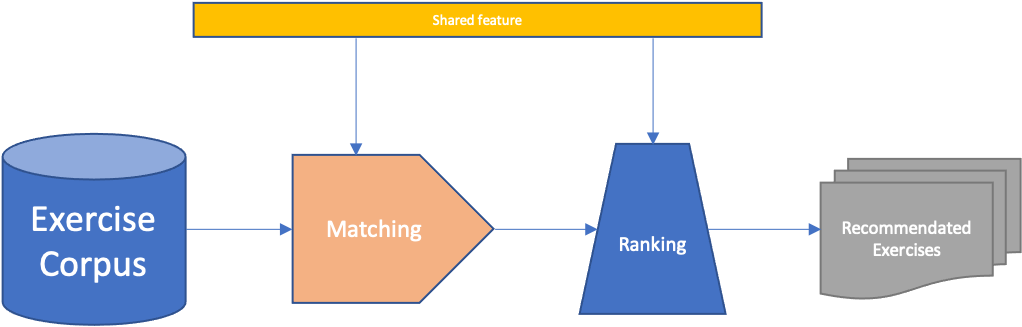
\includegraphics[width=1.0\textwidth]{ch4-fig-architecture.png }
  \caption{The Architecture of Recommendation System}\label{fig:ch4-fig0}
\end{figure}

\subsection{Matching Phase}
%本推荐模型的第一阶段为匹配,匹配层的目的是在确保一定准确度的情况下快速筛选出候选的推荐习题集合。匹配有多种策略来应对不同的应用场景。例如,与新闻推荐算法等相比,习题和用户的知识状态都是较为规则化的向量数据,计算习题、用户以及习题-用户交叉特征相似度相对简单,因此可以利用相似度匹配来应用协同过滤策略进行推荐项匹配。用户的历史回答错误错习题、统计的容易答错的习题等对于学生检查知识掌握完整度以及更正误区具有较大意义,因此筛选错误率较高的习题也可以作为一种匹配策略。在匹配阶段,可以应用不同的自适应参数或算法来控制候选习题集的大小,以适配原始数据集和推荐系统部署环境。

%采用不同的匹配策略,所对应的推荐侧重点也不同。一方面,不同的匹配策略会带来不同的推荐结果并忽略一部分推荐结果,例如,如果重视热门习题,则将做的人最多的习题作为匹配的结果,如果重视容易出错的习题,则将错误率较高的习题作为匹配的结果,如果重视基于相同兴趣的推荐,则将协同过滤作为匹配的结果。单独采用某一种匹配策略往往具有一定的缺陷,例如采用热门度作为匹配策略,会使得冷门习题几乎得不到被匹配的机会,导致推荐概率失衡,而采用错误率作为匹配策略则会无法匹配所有学生的知识情况。因此单独的匹配策略会丢失大量的推荐信息。另一方面,设计匹配层的时候,``计算速度''与``匹配率''这两个指标是相互矛盾的,也就是说在提高计算速度的时候需要尽量简化匹配策略,这就会导致匹配率不尽人意,同样的,需要提高匹配率时就需要复杂的匹配策略,这样计算速度肯定会相应的降低。在权衡两者后,目前工业界普遍采用多个简单的匹配策略叠加的``多路匹配策略''。``多路匹配策略''就是指采用不同的策略、特征或者简单模型,分别匹配一部分候选集,然后再把这些候选集进行合并、过滤等操作然后供后续排序模型使用的策略。多路匹配综合了多种匹配策略,结合了各个匹配策略的优点。在多路匹配中,每个策略之间毫不相关,所以一般可以写并发多线程同时进行。在实际的生产环境中,可以采取节点集群多线程地来进行召回操作,具备大规模商业应用的前景。

%本节提出一个多路习题推荐项匹配模型,该模型采用了基于热门度、用户兴趣、专家推荐习题、易错题、用户错题集和协同过滤等多个召回策略作为子召回策略,每个子召回策略都基于可学习的参数用于控制该召回策略的权重。当所有的召回策略都返回子召回习题集合后,通过基于加权融合的算法来进行习题的融合、过滤等步骤。其结构如图所示。

The first stage of this recommendation model is matching. The purpose of the matching layer is to quickly filter out a set of candidate recommended exercises while ensuring a certain degree of accuracy. There are multiple strategies for matching to deal with different application scenarios. For example, compared with news recommendation algorithms, the exercises and the user's knowledge state are more regularized vector data. It is relatively simple to calculate the similarity of exercises, users, and exercise-user cross-features, so similarity matching can be used to apply collaborative filtering. The strategy matches recommended items. The user's historical answers to wrong exercises and statistically easy to answer exercises are of great significance for students to check the completeness of their knowledge and correct their misunderstandings. Therefore, screening exercises with a higher error rate can also be used as a matching strategy. In the matching stage, different adaptive parameters or algorithms can be applied to control the size of the candidate problem set to adapt to the original data set and the recommended system deployment environment.

With different matching strategies, the corresponding recommendation focuses are also different. On the one hand, different matching strategies will lead to different recommendation results and ignore part of the recommendation results. For example, if the most popular exercises are emphasized, the exercises with the most people will be regarded as the matching results. If the exercises that are prone to errors are emphasized, errors will be regarded as the matching result. The exercises with a higher rate are used as the matching result. If the recommendation based on the same interest is emphasized, collaborative filtering will be used as the matching result. Adopting a certain matching strategy alone often has certain drawbacks. For example, using popularity as a matching strategy will make unpopular exercises almost impossible to be matched, resulting in an imbalance in the recommendation probability, while using error rate as a matching strategy will fail to match. Knowledge of all students. Therefore, a single matching strategy will lose a lot of recommendation information. On the other hand, when designing the matching layer, the two indicators of ``calculation speed'' and ``matching rate'' are contradictory. That is to say, the matching strategy needs to be simplified as much as possible when the calculation speed is increased. As a result, the matching rate is unsatisfactory. Similarly, when the matching rate needs to be improved, a complex matching strategy is required, so the calculation speed will definitely be reduced accordingly. After weighing the two, the current industry generally adopts a "multiplex matching strategy" in which multiple simple matching strategies are superimposed. The "multiplex matching strategy" refers to a strategy that uses different strategies, features or simple models to match a part of the candidate set, and then merges, filters, and other operations on these candidate sets, and then uses them for subsequent sorting models. multiplex matching integrates multiple matching strategies and combines the advantages of each matching strategy. In multiplex matching, each strategy is irrelevant, so it is generally possible to write concurrent multiple threads at the same time. In the actual production environment, the node cluster can be used for multi-threaded matching operations, which has the prospect of large-scale commercial applications.

This section proposes a multiplex exercise recommendation item matching model. The model uses multiple matching strategies based on popularity, user interest, expert recommendation exercises, error-prone questions, user error question sets, and collaborative filtering as sub-matching strategies. Matching strategies are based on learnable parameters to control the weight of the matching strategy. After all matching strategies have returned to the sub-matching exercise set, the exercises are merged and filtered through the algorithm based on weighted fusion. Its structure is shown in~\figurename{\ref{fig:ch4-matching-1}}.

\begin{figure}[h]
  \centering
  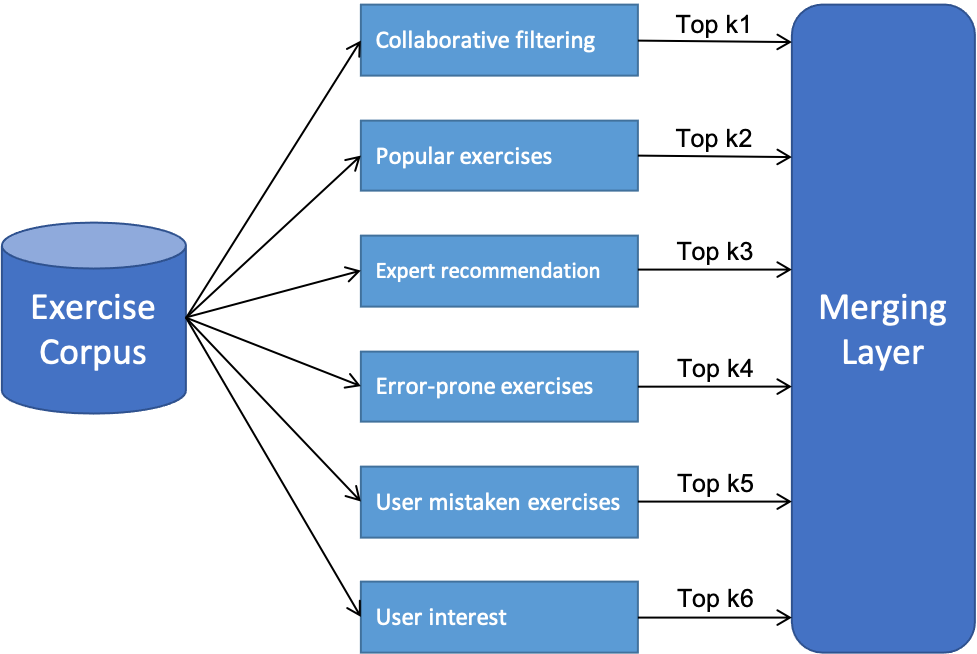
\includegraphics[width=1.0\textwidth]{ch4-matching-model1.png}
  \caption{The Multiplex Matching Method}\label{fig:ch4-matching-1}
\end{figure}

\subsubsection{Student-Exercise Collaborative Filtering}
%协同过滤是multiplex matching中的其中一个匹配策略,对于数学习题来说,由于习题已经经过知识点标注,因此可以根据知识点重合程度来计算相似度。同时,对于学生,在知识追踪阶段获取了学生的知识状态表征向量,因此也可以根据该向量计算学生的知识掌握相似度。本节提出一个基于Student-Exercise两阶段的协同过滤算法,该算法先计算学生的相似度,获取相关的习题,再根据这些习题计算相似的习题加入候选集,经过该方法计算的习题集相对而言较为完备,防止出现经过由于相似用户较少而出现的推荐项目稀疏的问题。

%传统基于用户的协同过滤根据模型选择的用户特征计算用户间的相似度,依据相似度来判定用户的状态相似度,并将相似度最高的前几名用户作为该用户的最近邻居用户,这些邻居用户构成目标用户的最近邻居用户集合。邻居用户集合的形成是之后推荐结果生成的重要前提和基础,对于相似用户的计算方法,目前大多数个性化推荐系统主要采用的有:余弦相似性、修正的余弦相似性、相关相似性,其中余弦相似性是计算两名用户评分向量在向量空 间模型中的向量夹角的余弦值,用评分向量夹角的余弦值大小表示用户间的相似性。而 修正的余弦相似性主要是解决用户受自身或者其它因素影响导致评分数据不稳定的问题,相较于余弦相似性计算用户间的相似度,修正的余弦相似性计算由于考虑因素较多 所以更为准确一些。

Collaborative filtering is one of the matching strategies in multiplex matching. For math learning questions, because the exercises have been labeled with knowledge points, the similarity can be calculated according to the degree of overlap of the knowledge points. At the same time, for students, the student's knowledge state representation vector is obtained in the knowledge tracking stage, so the similarity of the student's knowledge mastery can also be calculated based on the vector. This section proposes a two-stage collaborative filtering algorithm based on Student-Exercise. The algorithm first calculates the similarity of students, obtains related exercises, and then calculates similar exercises based on these exercises and adds them to the candidate set. The exercise set calculated by this method is relatively The language is relatively complete to prevent the problem of sparse recommendation items that have passed due to fewer similar users.

\subsubsection{Student Similarity Calculation}
%协同过滤的目的是向用户推荐与目标用户相似的推荐用户项目。通过用户的历史行为数据发现基于用户的协同过滤算法,并对这些偏好进行测量和评分。通过给定的算法设置用户的相似度,并在偏好相同的用户之间提出建议。

%基于用户的协同过滤主要考虑用户与用户之间的相似性。只要我们找出相似用户喜欢的项目并预测相应项目的目标用户评分,我们就可以找到评分最高的项目并将其推荐给用户。基于项目的协作过滤类似于基于用户的协作过滤,不同之处在于,我们转向查找项目与用户之间的相似性,并且只有当我们通过目标用户找到某些项目的评分时,我们才能通过高相似度,并向用户推荐评分最高的相似项。

%使用相似的统计数据来获得具有相似爱好或兴趣的邻近用户,因此我们可以使用从先前的知识跟踪模块中获得的用户的知识状态嵌入\(h_t\),可以将其用作计算相似性的基础。第一步是根据他们的历史行为信息找到与新用户相似的其他用户;同时,根据这些相似用户对其他商品的评价信息,预测当前新用户可能喜欢的商品。给定用户评分数据矩阵R,基于用户的协作过滤算法需要定义相似度函数\(s : U \times U \to R\)以计算用户之间的相似度,然后基于评分数据和相似度矩阵。我们可以使用余弦相似度来计算该值。


The purpose of collaborative filtering is to recommend recommended items of users similar to the target user to the user. The user-based collaborative filtering algorithm is discovered through historical behavior data of users, and measures and scores these preferences. Set the similarity of users through a given algorithm, and make recommendations among users who have the same preferences.

User-based collaborative filtering mainly considers the similarity between users and users. As long as we find out the items that similar users like and predict the target users' ratings of the corresponding items, we can find the items with the highest ratings and recommend them to users. The item-based collaborative filtering is similar to the user-based collaborative filtering, except that we turn to find the similarity between items and users, and only if we find the ratings of certain items by target users, then we can predict similar items with high similarity and recommend the highest rated similar items to users. For example, if you buy a machine learning related book online, the website will immediately recommend a bunch of machine learning, big data related books to you, and the idea of collaborative filtering based on items is obviously used here.

Similar statistics are used to get neighboring users with similar hobbies or interests, so we can use the obtained user's knowledge state embedding \(h_t\) from the previous knowledge tracking module, which can be used as the basis for calculating the similarity. The first step is to find other users who are similar to the new user based on their historical behavior information; at the same time, to predict the items that the current new user may like based on the evaluation information of these similar users on other items. Given the user rating data matrix R, the user-based collaborative filtering algorithm needs to define the similarity function \(s : U \times U \to R\) to calculate the similarity between users, and then calculate the recommendation results based on the rating data and the similarity matrix. We can use the cosine similarity to calculate this value.

\begin{align}
  s(u, v)=\frac{h_{u} \cdot h_{v}}{\|h_{u}\|_{2}\|h_{v}\|_{2}}
\end{align}
where \(h_u\) and \(h_v\) represent the knowledge mastery state of user \(u\) and \(v\).
We can obtain the exercise recommendation history \(\mathcal{H}\) of user B, which is closest to user A to be recommended, and then use the exercises in \(\mathcal{H}\) as a rough set as the next sorted list of exercises.

\subsubsection{Exercise Filtering System}
Through the previous section, we calculated the similarity of students, which comprehensively considers students' current knowledge proficiency, students' personalized information and so on. Next, we need to use the collaborative filtering algorithm to generate a rough recommended set of exercises \(S_{raw}\).

When the recommendation system is running, the system will record the students' question records. After calculating the similarity of the students, they can be sorted according to the similarity. Given a threshold, list the students whose similarity is greater than the threshold, and divide the students according to the list. The exercises corresponding to the problem record are added to \(S_{raw}\).

The algorithm is as~\ref{alg:EF}:
\begin{algorithm}[h]
  \caption{Exercise Filtering Algorithm}\label{alg:EF}
  \begin{algorithmic}
    \REQUIRE~~\\
    The target student \(s_i\); \\
    The student represent matrix, \(S=\{s_0,s_1,\ldots,s_N\} \);\\
    The log of recommendation \(L=\{L_0,L_1,\ldots,L_N\} \) \\
    The log-exercise relation: \(L_i=\{E_0,\ldots,E_{|L_i|}\} \) \\
    The filtering thread \(T\);
    \ENSURE~~\\ %算法的输出:Output
    The filtered exercise set \(S=\{E_{s_0},\ldots,E_{s_N}\} \)
    \STATE~Calculate the similarity between \(s_i\) and other students \(Sim\)
    \STATE~Sort \(Sim\) and get the top \(T\) results \(R=\{s_{r_0},\ldots,s_{r_T}\} \);
    \STATE~Aggregate the exercises log of students in \(R\), get exercise set \(S\)
    \RETURN~\(S\); %算法的返回值
  \end{algorithmic}
\end{algorithm}




\subsection{Ranking Stage}
%本节我们设计了一个基于MLP的试题排序模型,该模型输入学生的知识状态向量$h_t$,以及通过序列嵌入学习的知识状态改变向量$d_h$,以及习题的知识点标注向量。

In the previous step we obtained a list of recommended exercises for similar students by collaborative filtering in the matching phase, and in this phase, a ranking of the exercises is needed to further reduce the amount of recommendations and give the ranking sequence of exercise. In this section, we design an MLP-based test ordering model. The model inputs the student's knowledge state vector \(h_t\), the knowledge state change vector \(d_h\) learned through sequence embedding, and the knowledge point labeling vector of the exercises. The architecture is like \figurename{\ref{fig:ch4-fig3}}.


\begin{figure}[h]
  \centering
  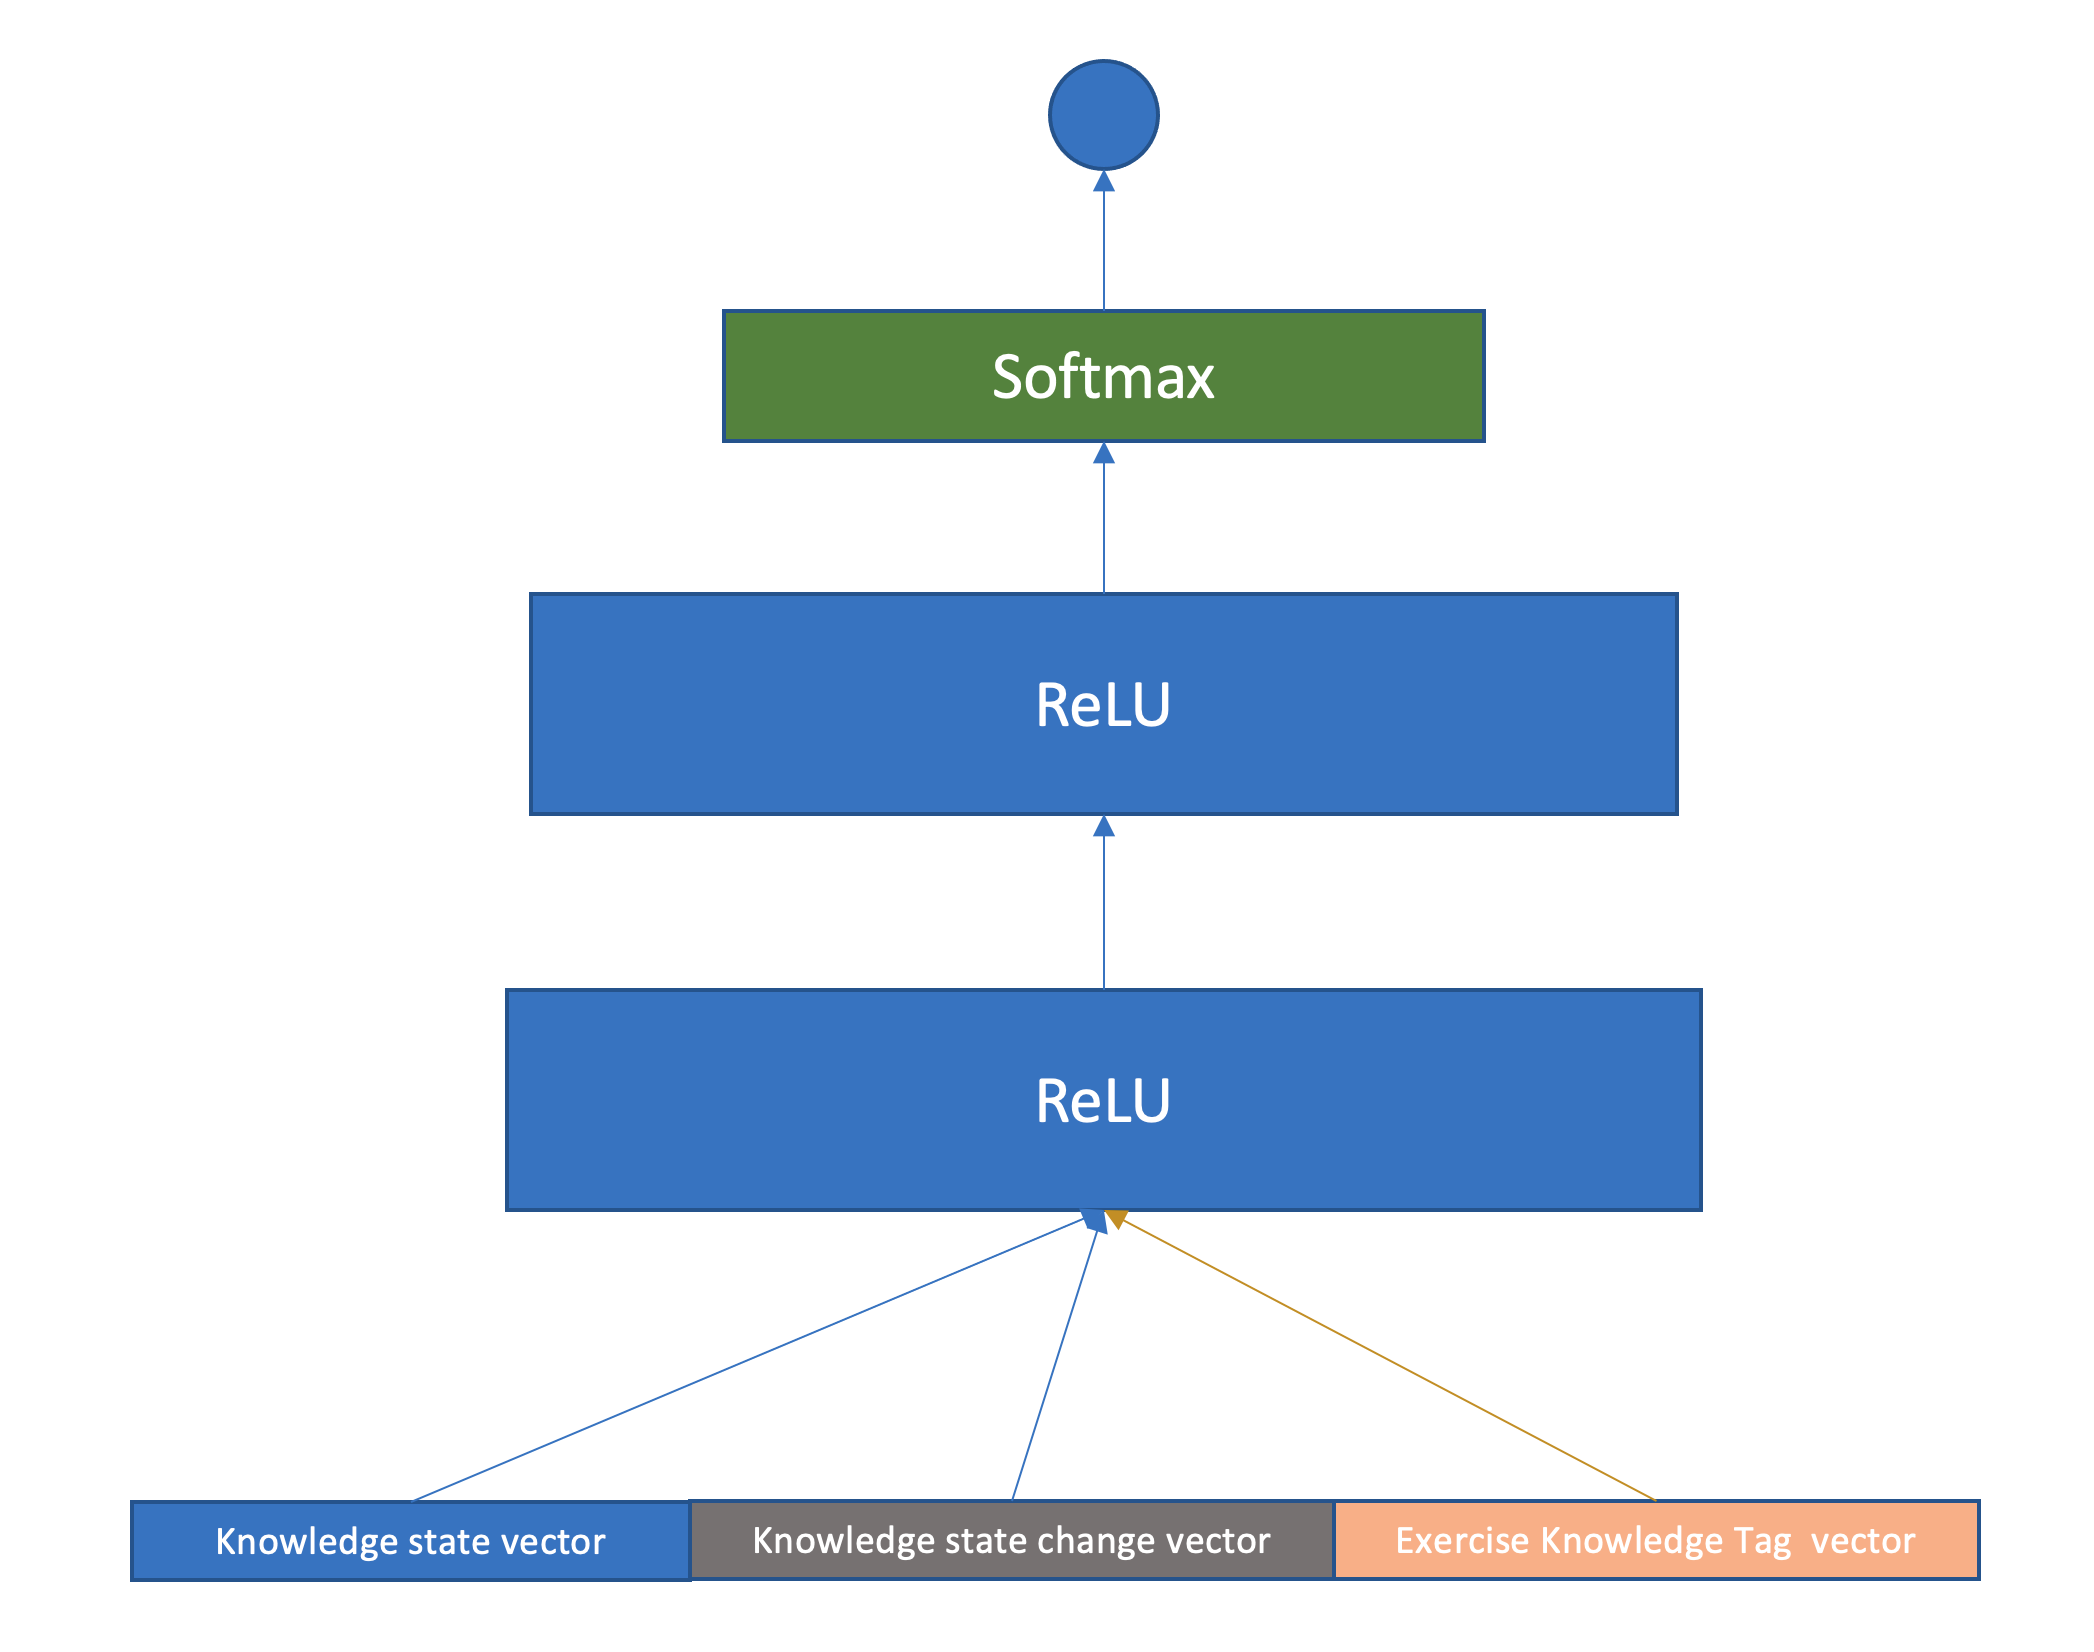
\includegraphics[width=1.0\textwidth]{ch4-fig3.png}
  \caption{The Architecture of Recommendation System}\label{fig:ch4-fig3}
\end{figure}

The model is a three-layer multi-layer perceptron, with two fully connected layers in the middle, and the output layer uses softmax to output the probabilities of exercise recommendation. The input layer inputs the student's knowledge state vector, knowledge state change vector and exercise knowledge point label vector. The model is a three-layer multi-layer perceptron, with two fully connected layers in the middle, and the output layer uses softmax to output the probabilities of exercise recommendation. The input layer inputs the student's knowledge state vector, knowledge state change vector and exercise knowledge point label vector. The loss function is:
\begin{align}
  \mathcal{L}=\sum_{i=1}^{T} y_i \log (\text{sigmoid}(\hat{y}_i))+(1-y_i ) \log (1-\text{sigmoid}(\hat{y}_i))
\end{align}
where \(\hat{y}_i\) is the output value, \(y_i\) is actual recommended weights for the exercises.

After training the model, sort the output values, and the sorted list is the recommended problem set.
%在训练好模型之后,将输出值进行排序,排序的列表即为推荐的习题集。


\section{Experiment}
%本模型的核心思想是为学生查漏补缺,因此,在学生的知识状态一定的情况下,尽量给学生推荐对其知识掌握情况带来正向收益最大的习题。
\subsection{Dataset}
%考虑到本推荐系统需要立足于学生的知识状态针对习题进行推荐。目前市面上并没有

\section{Summary}
%本节提出了一个基于匹配-排序的双阶段推荐系统框架,在匹配阶段,采用了协同过滤的方式,排序阶段,则采用了多层感知机,来对学生知识状态-习题知识点进行建模,同时考虑到学生的学习速度即知识状态改变,输出习题与当前知识状态匹配度。
This section proposes a two-stage recommendation system framework based on matching-ranking. In the matching stage, collaborative filtering is used, and in the ranking stage, multi-layer perceptron are used to model students' knowledge state-exercise knowledge points. At the same time, taking into account the student's learning speed, that is, the change of knowledge state, the output exercises match the current knowledge state.